% THIS IS SIGPROC-SP.TEX - VERSION 3.1
% WORKS WITH V3.2SP OF ACM_PROC_ARTICLE-SP.CLS
% APRIL 2009
%
% It is an example file showing how to use the 'acm_proc_article-sp.cls' V3.2SP
% LaTeX2e document class file for Conference Proceedings submissions.
% ----------------------------------------------------------------------------------------------------------------
% This .tex file (and associated .cls V3.2SP) *DOES NOT* produce:
%       1) The Permission Statement
%       2) The Conference (location) Info information
%       3) The Copyright Line with ACM data
%       4) Page numbering
% ---------------------------------------------------------------------------------------------------------------
% It is an example which *does* use the .bib file (from which the .bbl file
% is produced).
% REMEMBER HOWEVER: After having produced the .bbl file,
% and prior to final submission,
% you need to 'insert'  your .bbl file into your source .tex file so as to provide
% ONE 'self-contained' source file.
%
% Questions regarding SIGS should be sent to
% Adrienne Griscti ---> griscti@acm.org
%
% Questions/suggestions regarding the guidelines, .tex and .cls files, etc. to
% Gerald Murray ---> murray@hq.acm.org
%
% For tracking purposes - this is V3.1SP - APRIL 2009

\documentclass{acm_proc_article-sp}

\begin{document}

\title{Improving Data Collection and Monitoring through Dynamic Data Analysis}
\subtitle{}
%
% You need the command \numberofauthors to handle the 'placement
% and alignment' of the authors beneath the title.
%
% For aesthetic reasons, we recommend 'three authors at a time'
% i.e. three 'name/affiliation blocks' be placed beneath the title.
%
% NOTE: You are NOT restricted in how many 'rows' of
% "name/affiliations" may appear. We just ask that you restrict
% the number of 'columns' to three.
%
% Because of the available 'opening page real-estate'
% we ask you to refrain from putting more than six authors
% (two rows with three columns) beneath the article title.
% More than six makes the first-page appear very cluttered indeed.
%
% Use the \alignauthor commands to handle the names
% and affiliations for an 'aesthetic maximum' of six authors.
% Add names, affiliations, addresses for
% the seventh etc. author(s) as the argument for the
% \additionalauthors command.
% These 'additional authors' will be output/set for you
% without further effort on your part as the last section in
% the body of your article BEFORE References or any Appendices.

\numberofauthors{1} %  in this sample file, there are a *total*
% of EIGHT authors. SIX appear on the 'first-page' (for formatting
% reasons) and the remaining two appear in the \additionalauthors section.
%
\author{
% You can go ahead and credit any number of authors here,
% e.g. one 'row of three' or two rows (consisting of one row of three
% and a second row of one, two or three).
%
% The command \alignauthor (no curly braces needed) should
% precede each author name, affiliation/snail-mail address and
% e-mail address. Additionally, tag each line of
% affiliation/address with \affaddr, and tag the
% e-mail address with \email.
%
\alignauthor
P. Lubell-Doughtie, P. Pokharel, M. Johnston, V. Modi\\
       \affaddr{Columbia University}\\
       \affaddr{New York, New York}\\
       \email{pl2472@columbia.edu, prabhas.pokharel@gmail.com,
           mejymejy@gmail.com, modi@columbia.edu}
}
% Just remember to make sure that the TOTAL number of authors
% is the number that will appear on the first page PLUS the
% number that will appear in the \additionalauthors section.

\maketitle
\begin{abstract}
Feedback based on real-time data is seen as increasingly important for ICT-based interventions in the developing world. Applications such as real-time survey monitoring, real-time summarization of patient data based on community health worker, real-time outlier detection, and others need processes for analyzing, aggregating, and summarization of datasets that update over time. In order to facilitate such processes, we have created a modular web service for real-time data analysis: Bamboo.  Using a simple formula syntax, the Bamboo web service allows development planners to monitor data in real-time without a server infrastructure or in-house programmers.
\end{abstract}

% A category with the (minimum) three required fields
%\category{H.4}{Information Systems Applications}{Miscellaneous}
%A category including the fourth, optional field follows...
%\category{D.2.8}{Software Engineering}{Metrics}[complexity measures, performance measures]

%\terms{Theory}

%\keywords{ACM proceedings, \LaTeX, text tagging} % NOT required for Proceedings

\section{Introduction}
In order to effectively monitor health, allocate resources, and respond to crises both countries and planners need real-time data.  In mobile health systems, real-time monitoring can improve health programs and address key health risks [Mechael].  Real-time data can provide an audit trail that enables practitioners to learn how best to modify health programs and avert future deaths [Krisberg].  In emergency response, the time lag in processing of structured data causes significant delays; faster data analysis allows decisions makes address problems sooner and with greater impact [Internews].

However, dynamic data analysis requires resources and skills that are often unavailable in the development context.

Moreover, tools like EpiSurveyor, OpenDataKit / formhub.org allow development planners and others to conduct data gathering exercises without the need for server infrastrcture or in-house programmers. Even simplistic systems that perform custom user-defined aggregations and calculations on dynamic datasets, however, require server infrastructure and knowledge of general purpose programming languages. Bamboo aims to provide real-time aggregations, calculation, and summarization as a hosted web service, specified using an easy to learn formula syntax, and hosted as a web service so server infrastructure and/or programming skills are not required.

Bamboo was built as a tool to enable data analysis on data collected on the hosted data collection service formhub.org. The existing solutions before bamboo for performing dynamic data analysis were roughly categorized as:

custom tools, either built in-house or by a third-party, requiring server infrastructure e.g. based on LAMP stack, SQL
hosted tools, e.g. Google Fusion Tables or Google Docs
offline tools, e.g. R, Microsoft Excel, STATA, etc.

Custom tools are expensive and often beyond the capacity of most organizations; furthermore, they lead to duplication and are difficult to adapt to new tasks.  The hosted tools we evaluated had functional limitations that prevented their use.  For example, Google Fusion Tables only allows a limited set of calculations, and the one spreadsheet model of Google Docs precludes aggregations [Gonzalez:2010, Gonzalez:2010].  Offline tools have the flexibility required but have a steep learning curve and require a programmatic wrapper to allow for a truly dynamic workflow, thus creating a much higher barrier to entry.

\section{Design}
Bamboo sits between data collection and presentation. The dynamic statistical analysis within bamboo allows practitioners to easily build dashboards, maps, tables, and more which automatically update as new data arrives.  This enables the split-apply-combine strategy of data analysis [Wickham:2011] through a web service.

\begin{figure}
\centering
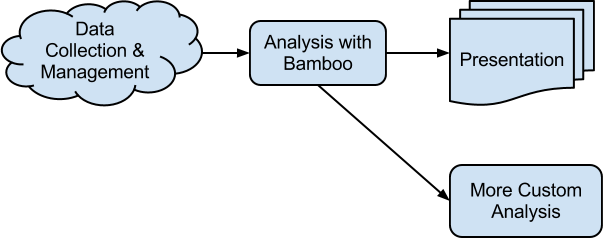
\includegraphics[width=3in]{figures/bamboo_flow}
\caption{Systematizing data collection and presentation with Bamboo.}
\end{figure}

Bamboo’s core functionality allows practitioners to:

\begin{itemize}
\item store, update, and merge data sets
\item build calculations and aggregations from data sets
\item generate summary statistics, means, counts, etc., from data sets
\end{itemize}

Generalizability is a fundamental principle of the design: Bamboo accepts any CSV file and provides users with complete control over the type of calculations.  To encourage community use and development we have made Bamboo open source and structured it to be easily extendable.  We also offer Bamboo as a hosted web service.  The Bamboo web service uses REST conventions and we have built client libraries that communicate with it in Python and JavaScript.

To serve as a general dynamic data analysis service, updates are propagated through the system ensuring that any aggregations or merged datasets are synchronized with the most recent data.

\begin{figure}
\centering
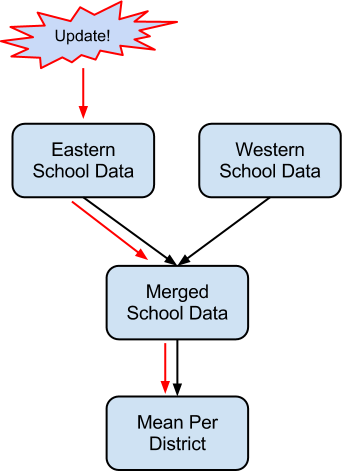
\includegraphics[width=2in]{figures/update_flow}
\caption{An update propagates from the dataset to all downstream merged datasets and aggregations.  The black arrows show structural dependencies created by the client.  The red arrow shows an update propagating through the system.}
\end{figure}

\subsection{Case Study 1: Survey Monitoring}

During a large data collection project in Nigeria, bamboo was used to monitor the progress of the surveying effort. By summarizing the amount of data collection per state and “facility type” [Figure 1], data collection monitors were able to identify states where data collection is lagging behind expectation.


Bamboo also allows exploratory analysis of this same dataset using more sophisticated 

For example, suppose you are an education minister monitoring school performance.  You decide to enter two datasets representing eastern and western school performance into the system and then combine them to produce a new merged data set.  Given that each dataset defines a num\_teachers column, this column will be available in calculations or aggregations.  Using a simple formula,

$$mean_num_teachers_by_district=mean(num_teachers), group=district$$

you can calculate the mean number of teachers per district for the merged dataset.

Now, what happens when new data for the eastern schools arrives?  With the aforementioned data analysis solutions, you would have to recombine your data and recalculate the mean per district.  Using Bamboo, you simply update the eastern school dataset and the system updates the merged dataset, automatically recalculating the mean per district given the new data.

\subsection{Case Study 2: Survey Monitoring}

Here we present a case study of how we have used Bamboo to assist in large scale data collection efforts.  During the surveying process it is important that data collection managers and government liaisons are able to monitor how the survey effort is progressing.  To fulfill these needs, we use Bamboo to create updatable histograms which display the amount of data that has been collected by each district and highlight where problems are.

[ histogram of districts, with some sucking]

The above histogram alerts data monitors that they should pay special attention to the Ogabaru [or whatever??] district.

To perform this analysis using an offline tool, we would need to:

\begin{enumerate}
\item export the data files
\item open each data file in desktop software
\item combine the datafiles into a single file
\item generate a chart
\item copy the chart to the web then email a link.
\end{enumerate}

The major disadvantage with this procedure is that all processes will have to be repeated each time the data is updated.

However, to perform the same analysis using bamboo we:

\begin{enumerate}
\item register a dataset with bamboo,
\item open up charts.bamboo.io using our dataset’s key,
\item and select the appropriate graph
\end{enumerate}

Even better, when the dataset is updated we only perform step (3).  The advantages are clear, there is no need to repeat previous tasks as new data arrives, we don’t need to keep track of files, and everything is recorded in one place.  What took five steps before can now be accomplished in a single step.

\section{Conclusions and Future Work}
Bamboo allows users without programming expertise to do dynamic data analysis.  Bamboo systematizes the process of creating indicators for domain specific data sets thereby reducing the time between collection and analysis, as well as the time between analysis and reporting.

In the future we will add additional analysis tools to encompass more real-world data processing tasks, such as levenshtein distance, nearest neighbors using k-means, time series analysis, and spatial analysis.  We plan to offer “calculation libraries” and allows users to build a set of calculations---e.g. health indicators---once, and then apply the same calculations to many datasets.

%\end{document}  % This is where a 'short' article might terminate

%
% The following two commands are all you need in the
% initial runs of your .tex file to
% produce the bibliography for the citations in your paper.
\bibliographystyle{abbrv}
\bibliography{acm_dev2013_mrg}  % sigproc.bib is the name of the Bibliography in this case
% You must have a proper ".bib" file
%  and remember to run:
% latex bibtex latex latex
% to resolve all references
%
% ACM needs 'a single self-contained file'!
%
%APPENDICES are optional
%\balancecolumns

\balancecolumns
% That's all folks!
\end{document}
